\section{User Simulation for System Evaluation}\label{sec:user_simulation}

One of the main challenges in developing conversational systems is the evaluation process. Testing with real users is expensive, time-consuming, and difficult to control due to numerous external variables. Moreover, unless participants are genuinely interested in purchasing a product, their responses may be biased or inconsistent, which undermines the objectivity of the evaluation. To address these challenges, we developed a simulated environment in which an LLM-based \textit{Simulated User Agent} plays the role of a human user and interacts with the chatbot system.


% \section{User Behaviour Simulation}
% Một trong những thách thức lớn nhất khi phát triển các hệ thống hội thoại là việc đánh giá hiệu quả. Việc thử nghiệm với người dùng thật tốn kém, mất thời gian và khó kiểm soát các biến số. Để khắc phục điều này, chúng tôi đã xây dựng một môi trường mô phỏng, trong đó một \textbf{Tác tử Người dùng (User Agent)} dựa trên LLM sẽ đóng vai người dùng để tương tác với chatbot.


\subsection{Simulated User Modeling for Interaction Testing}

To realistically simulate user behavior, the \textit{Simulated User Agent} makes decisions based on two primary inputs: (i) a fixed \textbf{User Profile} and (ii) the evolving \textbf{Dialogue Context}.

% \subsection{Thiết kế Tác tử Người dùng}
% Để mô phỏng hành vi của người dùng một cách thực tế, Tác tử Người dùng sử dụng hai thông tin đầu vào là (i) hồ sơ cá nhân và (ii) ngữ cảnh hội thoại để ra quyết định.

The \textbf{User Profile} remains constant throughout a session and comprises two key components: a \textit{user persona} and a \textit{synthetic interaction history}. The persona defines the user's behavioral archetype, such as a student, business professional, elderly user, or mobile gamer. Each persona is specified with detailed characteristics, shopping motivations, and decision patterns. For instance, a student persona is defined by a limited budget and high sensitivity to promotions.

The interaction history simulates prior purchases and inquiries, providing the agent with an initial set of interests before the conversation begins. This profile-driven structure supports more realistic and context-aware behavior as the dialogue unfolds.


% \textbf{Hồ sơ người dùng (User Profile)} được giữ cố định trong suốt một phiên hội thoại; nó bao gồm \textit{đặc điểm nhân vật} và \textit{lịch sử tương tác}. Để xây dựng \textit{đặc điểm nhân vật}, tác tử được chỉ định ngẫu nhiên để đóng một trong 10 vai trò người dùng khác nhau (ví dụ: Học sinh, Doanh nhân, Người lớn tuổi, Game thủ). Mỗi vai trò đi kèm với một mô tả chi tiết về đặc điểm, nhu cầu, và hành vi mua sắm. Ví dụ, một "Học sinh" sẽ có ngân sách hạn hẹp và quan tâm đến các chương trình khuyến mãi. Để xây dựng \textit{Lịch sử tương tác}, một lịch sử giả lập về các sản phẩm đã mua và đã hỏi trước đó được tạo ngẫu nhiên. Điều này giúp Tác tử Người dùng hình thành các mối quan tâm ban đầu trước khi bắt đầu cuộc trò chuyện.

The \textbf{Dialogue Context} captures the full conversation history, including the user's previous questions, the chatbot’s responses, and any suggested follow-up questions. The agent is instructed to prioritize the most recent question–answer exchanges in order to make context-aware decisions for the next turn.


% \textbf{Ngữ cảnh hội thoại (Conversation Context)} là toàn bộ lịch sử trò chuyện của người dùng, bao gồm câu hỏi trước đó, câu trả lời của chatbot và các gợi ý mới. Nó được yêu cầu tập trung vào những thông tin gần nhất để đưa ra quyết định tiếp theo.

Based on the User Profile and Dialogue Context, the Simulated User Agent selects one of two actions: \textbf{Accept}, by choosing a suggested follow-up question; or \textbf{Reject}, by ignoring all suggestions and generating a new question based on the character’s internal thoughts and needs.

To promote behavioral diversity and unpredictability, we set a high \texttt{temperature} value for the language model, enabling the agent to act in a more human-like and non-deterministic manner.


% Dựa trên hồ sơ người dùng và ngữ cảnh hội thoại, Tác tử Người dùng sẽ đưa ra một trong hai quyết định: \textbf{Chấp nhận (Accept)} -- Chọn một trong các câu hỏi được hệ thống gợi ý, hoặc (ii) \textbf{Từ chối (Reject)} -- Bỏ qua tất cả các gợi ý và tự tạo ra một câu hỏi mới dựa trên "suy nghĩ" và "nhu cầu" của nhân vật mà nó đang đóng vai.
% Chúng tôi thiết lập tham số \texttt{temperature} (mức độ sáng tạo) của LLM ở mức cao, giúp đảm bảo hành vi của Tác tử Người dùng có tính ngẫu nhiên và khó đoán, mô phỏng gần hơn với người dùng thật.

\subsection{User Simulation Flow and Termination Criteria}

A simulation session is a multi-turn conversation between the Simulated User Agent and the chatbot system. %The full interaction flow is illustrated in Figure~\ref{fig:simulation}. 
A session is labeled as a \textbf{success} if the user eventually asks about the target product. It is marked as a \textbf{failure} under either of the following conditions: (i) the number of dialogue turns exceeds a preset threshold (e.g., six turns) without reaching the target, or (ii) the Simulated User Agent rejects suggestions leading to the target product more than twice.

All user utterances, agent decisions, and intermediate system outputs are logged to support detailed analysis and system evaluation.

% \subsection{Luồng Mô phỏng và Điều kiện Dừng}
% Một phiên mô phỏng là một cuộc hội thoại nhiều lượt giữa Tác tử Người dùng và hệ thống chatbot. Luồng mô phỏng được thể hiện trong Hình \ref{fig:simulation}.
% Mỗi phiên mô phỏng sẽ kết thúc \textbf{Thành công (Success)} khi Tác tử Người dùng đặt một câu hỏi về sản phẩm mục tiêu, hoặc sẽ được xác định là \textbf{Thất bại (Fail)} khi hoặc (i) cuộc hội thoại vượt quá một số lượt nhất định (ví dụ, 6 lượt) mà vẫn chưa đạt được mục tiêu, hoặc (ii) tác tử Người dùng từ chối các gợi ý dẫn đến sản phẩm mục tiêu quá 2 lần.


% Toàn bộ cuộc hội thoại, các quyết định của Tác tử Người dùng, và các thông tin trung gian đều được ghi lại để phục vụ cho việc phân tích và lượng giá hiệu quả của hệ thống.

% \begin{figure*}[!t]
%     \centerline{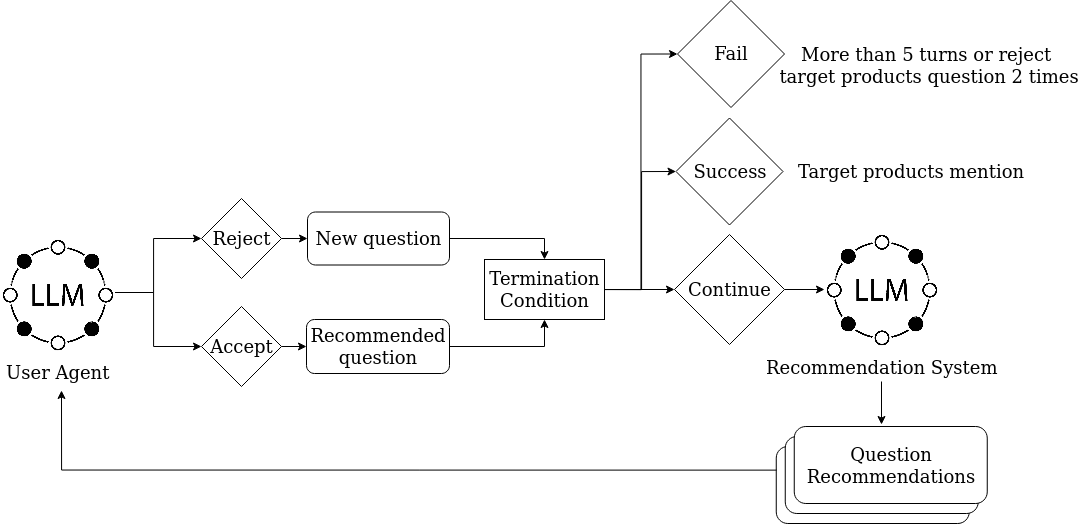
\includegraphics[width=\textwidth]{Figure/simulation_flow.png}}
%     \caption{Interaction flow of the User Simulation, detailing the Conversation Loop and Termination Conditions.}
%     \label{fig:simulation}
% \end{figure*}